%
% sampling.tex
%
% (c) 2019 Prof Dr Andreas Müller
%
\begin{frame}[fragile]
\frametitle{Sampling}

\begin{center}
\begin{tikzpicture}[>=latex]

	\def\stufe#1{
		\pgfmathparse{2*sin(15*(#1)*(12-(#1)))}
		\xdef\y{\pgfmathresult}
		\draw[color=red,line width=1pt] (\xold,\yold)--(#1,\yold);
		\draw[color=red,line width=0.1pt] (#1,\yold)--(#1,\y);
		\xdef\xold{#1}
		\xdef\yold{\y}
	}

	\draw[->,line width=0.7pt] (-0.1,0)--(12.6,0)
		coordinate[label={$t$}];
	\draw[->,line width=0.7pt] (0,-2.1)--(0,2.3)
		coordinate[label={right:$f$}];
	\draw[color=blue,line width=1pt] plot[domain=0:12.2,samples=1000]
		({\x},{2*sin(15*\x*(12-\x))});
	\def\xold{0}
	\def\yold{0}
	\only<1>{
		\foreach \x in {1,...,12}{ \stufe{\x} }
	}
	\only<2>{
		\foreach \x in {0.5,1,...,12}{ \stufe{\x} }
	}
	\only<3>{
		\foreach \x in {0.25,0.5,...,12}{ \stufe{\x} }
	}
	\only<4>{
		\foreach \x in {0.125,0.25,...,12}{ \stufe{\x} }
	}
	\only<5>{
		\foreach \x in {0.0625,0.125,...,12}{ \stufe{\x} }
	}
\end{tikzpicture}
\end{center}


\end{frame}




